% answers.tex —— 2016 年·全国Ⅰ卷·文科 · 参考答案与详细解析片段
% 由 tools/generate_projects.py 依来源总账自 2016/2016_数学真题_全国1文_试题.md + 2016/2016_数学真题_全国1文_解析正文.md + 2016/2016_数学真题_全国1文_答案要点.md 生成，勿手改（改源 MD 后重跑）


\begin{gktip}
以下解析依据固定原卷独立推导并经另一角色盲核，非官方解析。第 23 题按原题字面保留“所有公共点”的语义歧义，惯常非空交集解读单独注明。
\end{gktip}

\gkpart{选择题}

\begin{answer}
\gksolhead{1}{}

\textbf{题目}：

设集合 \(A=\{1,3,5,7\}\)，\(B=\{x\mid 2\leq x\leq 5\}\)，则 \(A\cap B=\)（　）

\begin{gkopts}(2)
\task （A）\(\{1,3\}\)
\task （B）\(\{3,5\}\)
\task （C）\(\{5,7\}\)
\task （D）\(\{1,7\}\)
\end{gkopts}

\Needspace{4\baselineskip}
\textbf{解析}

集合 \(A\) 中同时满足 \(2\le x\le5\) 的元素为 \(3,5\)，故交集为 \(\{3,5\}\)。

\gkanswer{答案：B，\(\{3,5\}\)}

\end{answer}
\begin{answer}
\gksolhead{2}{}

\textbf{题目}：

设 \((1+2i)(a+i)\) 的实部与虚部相等，其中 \(a\) 为实数，则 \(a=\)（　）

\begin{gkopts}(2)
\task （A）\(-3\)
\task （B）\(-2\)
\task （C）\(2\)
\task （D）\(3\)
\end{gkopts}

\Needspace{4\baselineskip}
\textbf{解析}

\nopagebreak[4]
\[
(1+2i)(a+i)=(a-2)+(2a+1)i.
\]
实部与虚部相等，故 \(a-2=2a+1\)，解得 \(a=-3\)。

\gkanswer{答案：A，\(-3\)}

\end{answer}
\begin{answer}
\gksolhead{3}{}

\textbf{题目}：

为美化环境，从红、黄、白、紫 4 种颜色的花中任选 2 种花种在一个花坛中，余下的 2 种花种在另一个花坛中，则红色和紫色的花不在同一花坛的概率是（　）

\begin{gkopts}(2)
\task （A）\(\dfrac{1}{3}\)
\task （B）\(\dfrac{1}{2}\)
\task （C）\(\dfrac{2}{3}\)
\task （D）\(\dfrac{5}{6}\)
\end{gkopts}

\Needspace{4\baselineskip}
\textbf{解析}

从四种花中选两种放进第一花坛，共有 \(\binom42=6\) 种等可能选择。红、紫分居两坛时，所选两种中恰有一种是红或紫，共 \(2\cdot2=4\) 种，因此所求概率为 \(\frac46=\frac23\)。

\gkanswer{答案：C，\(\frac23\)}

\end{answer}
\begin{answer}
\gksolhead{4}{}

\textbf{题目}：

\(\triangle ABC\) 的内角 \(A,B,C\) 的对边分别为 \(a,b,c\)。已知 \(a=\sqrt{5}\)，\(c=2\)，\(\cos A=\dfrac{2}{3}\)，则 \(b=\)（　）

\begin{gkopts}(2)
\task （A）\(\sqrt{2}\)
\task （B）\(\sqrt{3}\)
\task （C）\(2\)
\task （D）\(3\)
\end{gkopts}

\Needspace{4\baselineskip}
\textbf{解析}

\Needspace{5\baselineskip}
由余弦定理，
\nopagebreak[4]
\[
5=b^2+2^2-2\cdot b\cdot2\cdot\frac23,
\]
即 \(3b^2-8b-3=0\)。取正根得 \(b=3\)。

\gkanswer{答案：D，\(3\)}

\end{answer}
\begin{answer}
\gksolhead{5}{}

\textbf{题目}：

直线 \(l\) 经过椭圆的一个顶点和一个焦点，若椭圆中心到 \(l\) 的距离为其短轴长的 \(\dfrac{1}{4}\)，则该椭圆的离心率为（　）

\begin{gkopts}(2)
\task （A）\(\dfrac{1}{3}\)
\task （B）\(\dfrac{1}{2}\)
\task （C）\(\dfrac{2}{3}\)
\task （D）\(\dfrac{3}{4}\)
\end{gkopts}

\Needspace{4\baselineskip}
\textbf{解析}

\Needspace{5\baselineskip}
设椭圆半长轴、半短轴、半焦距分别为 \(a,b,c\)，则 \(a^2=b^2+c^2\)。短轴顶点 \((0,b)\) 与焦点 \((c,0)\) 的连线到中心的距离为
\nopagebreak[4]
\[
\frac{bc}{\sqrt{b^2+c^2}}=\frac{bc}{a}.
\]
题设使该距离为 \(b/2\)，所以 \(c/a=1/2\)，即离心率为 \(1/2\)。

\gkanswer{答案：B，\(\frac12\)}

\end{answer}
\begin{answer}
\gksolhead{6}{}

\textbf{题目}：

将函数 \(y=2\sin\left(2x+\dfrac{\pi}{6}\right)\) 的图象向右平移 \(\dfrac{1}{4}\) 个周期后，所得图象对应的函数为（　）

   （A）\(y=2\sin\left(2x+\dfrac{\pi}{4}\right)\)　（B）\(y=2\sin\left(2x+\dfrac{\pi}{3}\right)\)

   （C）\(y=2\sin\left(2x-\dfrac{\pi}{4}\right)\)　（D）\(y=2\sin\left(2x-\dfrac{\pi}{3}\right)\)

\Needspace{4\baselineskip}
\textbf{解析}

\Needspace{5\baselineskip}
原函数周期为 \(\pi\)，向右平移四分之一周期即平移 \(\pi/4\)。平移后的函数为
\nopagebreak[4]
\[
2\sin\left(2(x-\frac\pi4)+\frac\pi6\right)
=2\sin(2x-\frac\pi3).
\]

\gkanswer{答案：D，\(y=2\sin(2x-\frac\pi3)\)}

\end{answer}
\begin{answer}
\gksolhead{7}{}

\textbf{题目}：

如图，某几何体的三视图是三个半径相等的圆及每个圆中两条相互垂直的半径。若该几何体的体积是 \(\dfrac{28\pi}{3}\)，则它的表面积是（　）
\nopagebreak[4]
\begin{center}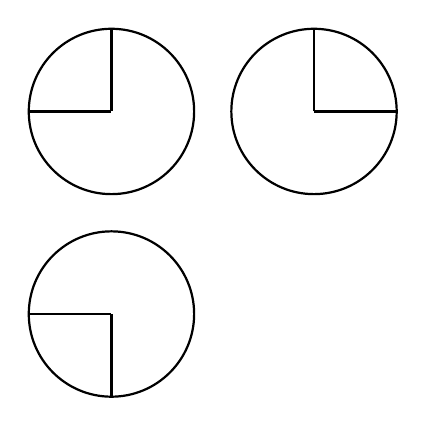
\begin{tikzpicture}[scale=1.05]
\draw[thick] (0,0) circle (1);
\draw[thick] (0,0) -- (0,1) (-1,0) -- (0,0);

\draw[thick] (2.45,0) circle (1);
\draw[thick] (2.45,0) -- (2.45,1) (2.45,0) -- (3.45,0);

\draw[thick] (0,-2.45) circle (1);
\draw[thick] (0,-2.45) -- (-1,-2.45) (0,-2.45) -- (0,-3.45);
\end{tikzpicture}
\end{center}
\nopagebreak[4]
\begin{gkopts}(2)
\task （A）\(17\pi\)
\task （B）\(18\pi\)
\task （C）\(20\pi\)
\task （D）\(28\pi\)
\end{gkopts}

\Needspace{4\baselineskip}
\textbf{解析}

\Needspace{5\baselineskip}
三视图表示半径为 \(r\) 的球去掉一个八分之一球体。由剩余体积
\nopagebreak[4]
\[
\frac78\cdot\frac43\pi r^3=\frac{28\pi}{3}
\]
得 \(r=2\)。球面部分面积为 \(\frac78\cdot4\pi r^2=14\pi\)；三个切面各为四分之一圆，合计 \(3\pi\)，故总表面积为 \(17\pi\)。

\gkanswer{答案：A，\(17\pi\)}

\end{answer}
\begin{answer}
\gksolhead{8}{}

\textbf{题目}：

若 \(a>b>0\)，\(0<c<1\)，则（　）

   （A）\(\log_a c<\log_b c\)　（B）\(\log_c a<\log_c b\)

   （C）\(a^c<b^c\)　（D）\(c^a>c^b\)

\Needspace{4\baselineskip}
\textbf{解析}

因 \(0<c<1\)，函数 \(\log_c x\) 递减。由 \(a>b>0\) 得 \(\log_c a<\log_c b\)。

\gkanswer{答案：B，\(\log_c a<\log_c b\)}

\end{answer}
\begin{answer}
\gksolhead{9}{}

\textbf{题目}：

函数 \(y=2x^2-e^{|x|}\) 在 \([-2,2]\) 的图象大致为（　）
\nopagebreak[4]
\begin{center}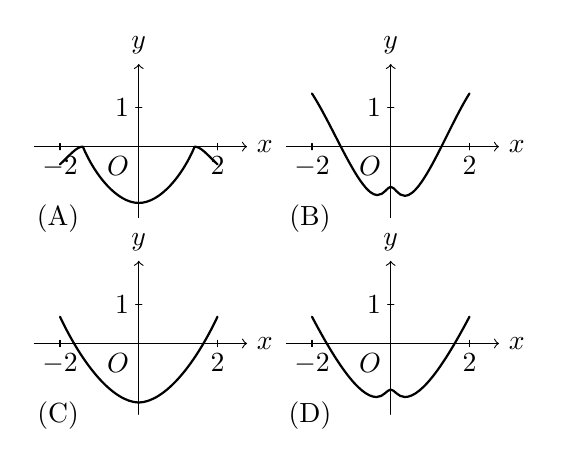
\begin{tikzpicture}[x=0.5cm,y=0.5cm,line cap=round,line join=round]
\begin{scope}
  \draw[->] (-2.65,0) -- (2.75,0) node[right] {$x$};
  \draw[->] (0,-1.8) -- (0,2.1) node[above] {$y$};
  \draw (-2,0.08) -- (-2,-0.08) (2,0.08) -- (2,-0.08);
  \draw (0.08,1) -- (-0.08,1);
  \node[below] at (-2,0) {$-2$};
  \node[below] at (2,0) {$2$};
  \node[left] at (0,1) {$1$};
  \node[below left] at (0,0) {$O$};
  \draw[thick] (-2,-0.45)
    .. controls (-1.72,-0.18) and (-1.57,0) .. (-1.42,0)
    .. controls (-1.12,-0.72) and (-0.55,-1.43) .. (0,-1.43)
    .. controls (0.55,-1.43) and (1.12,-0.72) .. (1.42,0)
    .. controls (1.57,0) and (1.72,-0.18) .. (2,-0.45);
  \node at (-2.05,-1.83) {(A)};
\end{scope}

\begin{scope}[shift={(6.4,0)}]
  \draw[->] (-2.65,0) -- (2.75,0) node[right] {$x$};
  \draw[->] (0,-1.8) -- (0,2.1) node[above] {$y$};
  \draw (-2,0.08) -- (-2,-0.08) (2,0.08) -- (2,-0.08);
  \draw (0.08,1) -- (-0.08,1);
  \node[below] at (-2,0) {$-2$};
  \node[below] at (2,0) {$2$};
  \node[left] at (0,1) {$1$};
  \node[below left] at (0,0) {$O$};
  \draw[thick] (-2,1.35)
    .. controls (-1.43,0.47) and (-0.79,-1.23) .. (-0.34,-1.23)
    .. controls (-0.17,-1.23) and (-0.08,-1.02) .. (0,-1.02)
    .. controls (0.10,-1.02) and (0.18,-1.25) .. (0.36,-1.25)
    .. controls (0.82,-1.25) and (1.45,0.48) .. (2,1.35);
  \node at (-2.05,-1.83) {(B)};
\end{scope}

\begin{scope}[shift={(0,-5)}]
  \draw[->] (-2.65,0) -- (2.75,0) node[right] {$x$};
  \draw[->] (0,-1.8) -- (0,2.1) node[above] {$y$};
  \draw (-2,0.08) -- (-2,-0.08) (2,0.08) -- (2,-0.08);
  \draw (0.08,1) -- (-0.08,1);
  \node[below] at (-2,0) {$-2$};
  \node[below] at (2,0) {$2$};
  \node[left] at (0,1) {$1$};
  \node[below left] at (0,0) {$O$};
  \draw[thick] (-2,0.68)
    .. controls (-1.42,-0.55) and (-0.66,-1.48) .. (0,-1.5)
    .. controls (0.66,-1.48) and (1.42,-0.55) .. (2,0.68);
  \node at (-2.05,-1.83) {(C)};
\end{scope}

\begin{scope}[shift={(6.4,-5)}]
  \draw[->] (-2.65,0) -- (2.75,0) node[right] {$x$};
  \draw[->] (0,-1.8) -- (0,2.1) node[above] {$y$};
  \draw (-2,0.08) -- (-2,-0.08) (2,0.08) -- (2,-0.08);
  \draw (0.08,1) -- (-0.08,1);
  \node[below] at (-2,0) {$-2$};
  \node[below] at (2,0) {$2$};
  \node[left] at (0,1) {$1$};
  \node[below left] at (0,0) {$O$};
  \draw[thick] (-2,0.68)
    .. controls (-1.43,-0.40) and (-0.82,-1.36) .. (-0.36,-1.36)
    .. controls (-0.18,-1.36) and (-0.09,-1.17) .. (0,-1.17)
    .. controls (0.09,-1.17) and (0.18,-1.36) .. (0.36,-1.36)
    .. controls (0.82,-1.36) and (1.43,-0.40) .. (2,0.68);
  \node at (-2.05,-1.83) {(D)};
\end{scope}
\end{tikzpicture}
\end{center}
\nopagebreak[4]
\Needspace{4\baselineskip}
\textbf{解析}

\Needspace{5\baselineskip}
函数 \(f(x)=2x^2-e^{|x|}\) 为偶函数，且 \(f(0)=-1\)。在 \(x>0\) 时
\nopagebreak[4]
\[
f'(x)=4x-e^x.
\]
令 \(h(x)=4x-e^x\)。在 \([0,1]\) 上 \(h'(x)=4-e^x>0\)，而 \(h(0)=-1<0<h(1)=4-e\)，故有唯一零点；在 \([1,2]\) 上，\(h\) 为凹函数且两端点值均为正（\(h(1)=4-e,\ h(2)=8-e^2\)），故仍为正。于是原点为尖点局部极大值，两侧各有一个局部极小值，图象关于 \(y\) 轴对称且端点 \(x=\pm2\) 处高于零，符合选项 D。

\gkanswer{答案：D}

\end{answer}
\begin{answer}
\gksolhead{10}{}

\textbf{题目}：

执行下面的程序图，如果输入的 \(x=0,y=1,n=1\)，则输出 \(x,y\) 的值满足（　）
\nopagebreak[4]
\begin{center}\begin{tikzpicture}[line cap=round,line join=round]
% 开始与输入
\draw[rounded corners=3pt] (-0.65,6.3) rectangle (0.65,6.9);
\node at (0,6.6) {开始};
\draw (-1.55,5.3) -- (1.25,5.3) -- (1.55,4.65) -- (-1.25,4.65) -- cycle;
\node at (0,4.98) {输入 $x,y,n$};
\draw[->] (0,6.3) -- (0,5.3);

% 更新与循环判断
\draw (-2.75,3.15) rectangle (2.75,4.25);
\node at (0,3.85) {$x=x+\dfrac{n-1}{2},\quad y=ny$};
\draw (0,4.65) -- (0,4.48);
\draw[->] (0,4.48) -- (0,4.25);

\draw (0,1.95) -- (2.15,1.45) -- (0,0.95) -- (-2.15,1.45) -- cycle;
\node at (0,1.45) {$x^2+y^2\geq 36$};
\draw[->] (0,3.15) -- (0,1.95);

% 否分支先递增 n，再返回更新框
\draw (-4.9,2.3) rectangle (-2.7,2.8);
\node at (-3.8,2.55) {$n=n+1$};
\draw (-2.15,1.45) -- (-3.8,1.45);
\draw[->] (-3.8,1.45) -- (-3.8,2.3);
\draw[->] (-3.8,2.8) -- (-3.8,4.48);
\draw[->] (-3.8,4.48) -- (0,4.48);
\node at (-2.65,1.2) {否};

% 是分支输出并结束
\draw (-1.3,0.25) -- (1.3,0.25) -- (1.05,-0.45) -- (-1.55,-0.45) -- cycle;
\draw[->] (0,0.95) -- (0,0.25);
\node at (-0.38,0.68) {是};
\node at (-0.25,-0.1) {输出 $x,y$};
\draw[->] (0,-0.45) -- (0,-0.85);
\draw[rounded corners=3pt] (-0.65,-1.45) rectangle (0.65,-0.85);
\node at (0,-1.15) {结束};
\end{tikzpicture}
\end{center}
\nopagebreak[4]
\begin{gkopts}(2)
\task （A）\(y=2x\)
\task （B）\(y=3x\)
\task （C）\(y=4x\)
\task （D）\(y=5x\)
\end{gkopts}

\Needspace{4\baselineskip}
\textbf{解析}

第一次按 \(n=1\) 更新后仍为 \((x,y,n)=(0,1,1)\)，尚未达到阈值；随后令 \(n=2\)，更新得到 \((x,y,n)=(\frac12,2,2)\)，仍未达到阈值。再令 \(n=3\)，更新得 \((\frac32,6,3)\)，此时 \(x^2+y^2=38.25\ge36\)，停止。输出满足 \(y=4x\)。

\gkanswer{答案：C，\(y=4x\)}

\end{answer}
\begin{answer}
\gksolhead{11}{}

\textbf{题目}：

平面 \(\alpha\) 过正方体 \(ABCD-A_1B_1C_1D_1\) 的顶点 \(A\)，\(\alpha\parallel\) 平面 \(CB_1D_1\)，\(\alpha\cap\) 平面 \(ABCD=m\)，\(\alpha\cap\) 平面 \(ABB_1A_1=n\)，则 \(m,n\) 所成角的正弦值为（　）

\begin{gkopts}(2)
\task （A）\(\dfrac{\sqrt{3}}{2}\)
\task （B）\(\dfrac{\sqrt{2}}{2}\)
\task （C）\(\dfrac{\sqrt{3}}{3}\)
\task （D）\(\dfrac{1}{3}\)
\end{gkopts}

\Needspace{4\baselineskip}
\textbf{解析}

取正方体棱长为 \(1\)，令 \(A=(0,0,0)\)、\(B=(1,0,0)\)、\(C=(1,1,0)\)、\(B_1=(1,0,1)\)、\(D_1=(0,1,1)\)。平面 \(CB_1D_1\) 的方程为 \(x+y+z=2\)，过 \(A\) 的平行平面为 \(x+y+z=0\)。该平面与底面、侧面 \(ABB_1A_1\) 的交线方向分别可取 \((1,-1,0)\)、\((1,0,-1)\)，夹角余弦的绝对值为 \(1/2\)，故锐角正弦为 \(\sqrt3/2\)。

\gkanswer{答案：A，\(\frac{\sqrt3}{2}\)}

\end{answer}
\begin{answer}
\gksolhead{12}{}

\textbf{题目}：

若函数 \(f(x)=x-\dfrac{1}{3}\sin 2x+a\sin x\) 在 \(( -\infty,+\infty )\) 单调递增，则 \(a\) 的取值范围是（　）

\begin{gkopts}(1)
\task （A）\([-1,1]\)
\task （B）\([-1,\dfrac{1}{3}]\)
\task （C）\([-\dfrac{1}{3},\dfrac{1}{3}]\)
\task （D）\([-1,-\dfrac{1}{3}]\)
\end{gkopts}

\Needspace{4\baselineskip}
\textbf{解析}

\Needspace{5\baselineskip}
令 \(t=\cos x\in[-1,1]\)，则
\nopagebreak[4]
\[
f'(x)=1-\frac23\cos2x+a\cos x
=\frac{5-4t^2+3at}{3}.
\]
右侧为关于 \(t\) 的凹二次函数，在闭区间上的最小值取于端点。两端非负分别要求 \(a\ge-\frac13\)、\(a\le\frac13\)，所以 \(a\in[-\frac13,\frac13]\)。

\gkanswer{答案：C，\([-\frac13,\frac13]\)}

\end{answer}
\gkpart{填空题}

\begin{answer}
\gksolhead{13}{}

\textbf{题目}：

设向量 \(\boldsymbol{a}=(x,x+1)\)，\(\boldsymbol{b}=(1,2)\)，且 \(\boldsymbol{a}\perp\boldsymbol{b}\)，则 \(x=\)\gkblank{}。

\Needspace{4\baselineskip}
\textbf{解析}

垂直条件给出 \((x,x+1)\cdot(1,2)=0\)，即 \(3x+2=0\)，故 \(x=-\frac23\)。

\gkanswer{答案：\(-\frac23\)}

\end{answer}
\begin{answer}
\gksolhead{14}{}

\textbf{题目}：

已知 \(\theta\) 是第四象限角，且 \(\sin\left(\theta+\dfrac{\pi}{4}\right)=\dfrac{3}{5}\)，则 \(\tan\left(\theta-\dfrac{\pi}{4}\right)=\)\gkblank{}。

\Needspace{4\baselineskip}
\textbf{解析}

\Needspace{5\baselineskip}
令 \(\phi=\theta+\frac\pi4\)。由象限条件 \(\phi\in(0,\frac\pi4)\)，且 \(\sin\phi=\frac35,\cos\phi=\frac45\)。于是
\nopagebreak[4]
\[
\tan(\theta-\frac\pi4)=\tan(\phi-\frac\pi2)=-\cot\phi=-\frac43.
\]

\gkanswer{答案：\(-\frac43\)}

\end{answer}
\begin{answer}
\gksolhead{15}{}

\textbf{题目}：

设直线 \(y=x+2a\) 与圆 \(C:x^2+y^2-2ay-2=0\) 相交于 \(A,B\) 两点，若 \(|AB|=2\sqrt{3}\)，则圆 \(C\) 的面积为\gkblank{}。

\Needspace{4\baselineskip}
\textbf{解析}

\Needspace{5\baselineskip}
圆心为 \((0,a)\)，半径平方为 \(a^2+2\)。圆心到直线 \(y=x+2a\) 的距离为 \(|a|/\sqrt2\)。由弦长公式，半弦长平方满足
\nopagebreak[4]
\[
a^2+2-\frac{a^2}{2}=3,
\]
所以 \(a^2=2\)，圆半径平方为 \(4\)，面积为 \(4\pi\)。

\gkanswer{答案：\(4\pi\)}

\end{answer}
\begin{answer}
\gksolhead{16}{}

\textbf{题目}：

某高科技企业生产产品 \(A\) 和产品 \(B\)，需要甲、乙两种新型材料。生产一件产品 \(A\) 需要甲材料 \(1.5\ \mathrm{kg}\)、乙材料 \(1\ \mathrm{kg}\)，用 5 个工时；生产一件产品 \(B\) 需要甲材料 \(0.5\ \mathrm{kg}\)、乙材料 \(0.3\ \mathrm{kg}\)，用 3 个工时；生产一件产品 \(A\) 的利润为 2100 元，生产一件产品 \(B\) 的利润为 900 元。该企业现有甲材料 150 kg、乙材料 90 kg，则在不超过 600 个工时的条件下，生产产品 \(A\)、产品 \(B\) 的利润之和的最大值为\gkblank{}元。

\Needspace{4\baselineskip}
\textbf{解析}

\Needspace{5\baselineskip}
设两种产品产量为 \(x,y\)。原料与工时约束化为
\nopagebreak[4]
\[
3x+y\le300,\quad10x+3y\le900,\quad5x+3y\le600,\quad x,y\ge0.
\]
可行域顶点为 \((0,0),(90,0),(60,100),(0,200)\)。

目标函数 \(2100x+900y\) 在这些点分别为 \(0,189000,216000,180000\)，最大值为 \(216000\) 元。

\gkanswer{答案：\(216000\) 元}

\end{answer}
\gkpart{解答题}

\begin{answer}
\gksolhead{17}{}

\textbf{题目}：

已知 \(\{a_n\}\) 是公差为 3 的等差数列，数列 \(\{b_n\}\) 满足 \(b_1=1\)，\(b_2=\dfrac{1}{3}\)，\(a_nb_{n+1}+b_{n+1}=nb_n\)。

   （1）　求 \(\{a_n\}\) 的通项公式；

   （2）　求 \(\{b_n\}\) 的前 \(n\) 项和。

\Needspace{4\baselineskip}
\textbf{解析}

\gksubpart{(1)}

递推式在 \(n=1\) 时给出 \((a_1+1)b_2=b_1\)。代入 \(b_1=1,b_2=\frac13\)，得 \(a_1=2\)。公差为 \(3\)，所以 \(a_n=2+3(n-1)=3n-1\)。

\gksubpart{(2)}

\Needspace{5\baselineskip}
代入递推式 \((a_n+1)b_{n+1}=nb_n\)，并用 \(a_n=3n-1\)，得 \(3nb_{n+1}=nb_n\)，故 \(b_{n+1}=b_n/3\)。于是 \(b_n=3^{-(n-1)}\)，从而
\nopagebreak[4]
\[
S_n=\sum_{k=1}^n3^{-(k-1)}=\frac32(1-3^{-n}).
\]

\gkanswer{答案（1）：\(a_n=3n-1\)}

\gkanswer{答案（2）：\(S_n=\frac32(1-3^{-n})\)}

\end{answer}
\begin{answer}
\gksolhead{18}{}

\textbf{题目}：

如图，在已知正三棱锥 \(P-ABC\) 的侧面是直角三角形，\(PA=6\)，顶点 \(P\) 在平面 \(ABC\) 内的正投影为点 \(D\)，\(D\) 在平面 \(PAB\) 内的正投影为点 \(E\)，连接 \(PE\) 并延长交 \(AB\) 于点 \(G\)。
\nopagebreak[4]
\begin{center}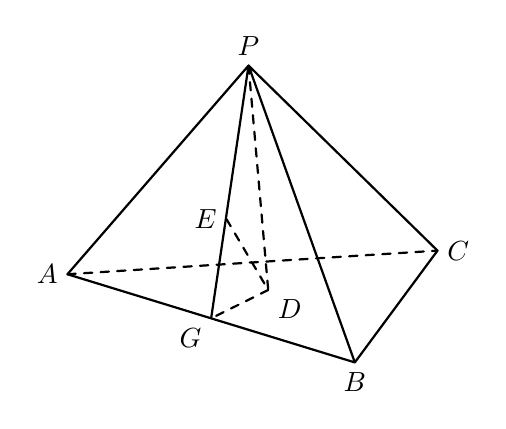
\begin{tikzpicture}[line cap=round,line join=round]
\coordinate (A) at (0,0);
\coordinate (B) at (3.65,-1.12);
\coordinate (C) at (4.7,0.3);
\coordinate (P) at (2.3,2.65);
\coordinate (G) at (1.825,-0.56);
\coordinate (E) at (2.02,0.70);
\coordinate (D) at (2.55,-0.20);

% 隐线与内部构造
\draw[thick,dashed] (A)--(C) (P)--(D) (E)--(D) (D)--(G);
% 棱与 PE 延长线 PG
\draw[thick] (A)--(B)--(C) (A)--(P) (B)--(P) (C)--(P) (P)--(G);

\node[left] at (A) {$A$};
\node[below] at (B) {$B$};
\node[right] at (C) {$C$};
\node[above] at (P) {$P$};
\node[left] at (E) {$E$};
\node[below right] at (D) {$D$};
\node[below left] at (G) {$G$};
\end{tikzpicture}
\end{center}
\nopagebreak[4]
   （1）　证明 \(G\) 是 \(AB\) 的中点；

   （2）　如图，在图中作出点 \(E\) 在平面 \(PAC\) 内的正投影 \(F\)（说明做法及理由），并求四面体 \(PDEF\) 的体积。

\Needspace{4\baselineskip}
\textbf{解析}

\Needspace{5\baselineskip}
侧面为直角等腰三角形且 \(PA=6\)，故 \(PA=PB=PC=6\)，底边长均为 \(6\sqrt2\)。取
\nopagebreak[4]
\[
A=(-3\sqrt2,0,0),\ B=(3\sqrt2,0,0),\ C=(0,3\sqrt6,0),\
D=(0,\sqrt6,0),\ P=(0,\sqrt6,2\sqrt3).
\]

\gksubpart{(1)}

正三棱锥的对称面经过顶点 \(P\)、底面重心 \(D\) 与 \(AB\) 中点 \(G\)，并保持平面 \(PAB\) 不变。由于 \(D\) 在对称面内，其在平面 \(PAB\) 上的正投影 \(E\) 也在该对称面内；因此 \(PE\) 与 \(AB\) 的交点为中点 \(G\)。

\gksubpart{(2)}

在平面 \(PAB\) 内作 \(EK\perp PA\)，过 \(E\) 作与 \(PA\) 垂直的截面 \(\Sigma\)，令 \(\ell=\Sigma\cap\text{平面 }PAC\)；再在 \(\Sigma\) 内过 \(E\) 作 \(EF\perp\ell\)。因为 \(PA\perp\Sigma\)，所以 \(EF\perp PA\) 且 \(EF\perp\ell\)；而 \(PA,\ell\) 张成平面 \(PAC\)，故 \(EF\perp\text{平面 }PAC\)，\\
\(F\) 即所求正投影。

平面 \(PAB\) 的法向量可取 \((0,-\sqrt2,1)\)，投影得 \(E=(0,\frac{\sqrt6}{3},\frac{2\sqrt3}{3})\)。

\Needspace{5\baselineskip}
平面 \(PAC\) 的法向量可取 \((3\sqrt2,-\sqrt6,-2\sqrt3)\)，将 \(E\) 正投影到该平面得
\nopagebreak[4]
\[
F=(-\sqrt2,\frac{2\sqrt6}{3},\frac{4\sqrt3}{3}).
\]
\Needspace{5\baselineskip}
于是四面体体积
\nopagebreak[4]
\[
V_{PDEF}=\frac16\left|(D-P)\cdot((E-P)\times(F-P))\right|=\frac86=\frac43.
\]

\gkanswer{答案（1）：\(G\) 为 \(AB\) 中点}

\gkanswer{答案（2）：\(F\) 是 \(E\) 在平面 \(PAC\) 上的正投影，\(V_{PDEF}=\frac43\)}

\end{answer}
\begin{answer}
\gksolhead{19}{}

\textbf{题目}：

某公司计划购买 1 台机器，该种机器使用三年后即被淘汰，机器有一易损零件。在购进机器时，可以额外购买这种零件作为备件，每个 200 元。在机器使用期间，如果备件不足再购买，则每个 500 元。现需决策在购买机器时应同时购买几个易损零件，为此搜集并整理了 100 台这种机器在三年试用期内更换的易损零件数，得下面柱状图：
\nopagebreak[4]
\begin{center}\begin{tikzpicture}[x=0.92cm,y=0.15cm,line cap=butt,line join=round]
% 频数轴与横轴
\draw[->,thick] (0,0) -- (0,27.2);
\draw[->,thick] (0,0) -- (7.05,0);
\node[above right] at (0,26.1) {频数};
\node[below left] at (0,0) {$0$};

% 频数参考虚线，延伸到对应柱的左边缘
\draw[dashed] (0,6) -- (0.72,6);
\draw[dashed] (0,10) -- (5.72,10);
\draw[dashed] (0,16) -- (1.72,16);
\draw[dashed] (0,20) -- (4.72,20);
\draw[dashed] (0,24) -- (2.72,24);
\node[left] at (0,6) {$6$};
\node[left] at (0,10) {$10$};
\node[left] at (0,16) {$16$};
\node[left] at (0,20) {$20$};
\node[left] at (0,24) {$24$};

% 16 至 21 的频数依次为 6、16、24、24、20、10
\draw (0.72,0) rectangle (1.28,6);
\draw (1.72,0) rectangle (2.28,16);
\draw (2.72,0) rectangle (3.28,24);
\draw (3.72,0) rectangle (4.28,24);
\draw (4.72,0) rectangle (5.28,20);
\draw (5.72,0) rectangle (6.28,10);

% 横轴断轴符号与类别刻度
\draw[thick] (0.10,-0.55) -- (0.18,0.55) -- (0.26,-0.55) -- (0.34,0.55) -- (0.42,-0.55);
\node[below=3pt] at (1,0) {$16$};
\node[below=3pt] at (2,0) {$17$};
\node[below=3pt] at (3,0) {$18$};
\node[below=3pt] at (4,0) {$19$};
\node[below=3pt] at (5,0) {$20$};
\node[below=3pt] at (6,0) {$21$};
\node[above right] at (6.8,0) {更换的易损零件数};
\end{tikzpicture}
\end{center}
\nopagebreak[4]
   记 \(x\) 表示 1 台机器在三年试用期内需更换的易损零件数，\(y\) 表示 1 台机器在购买易损零件上所需的费用（单位：元），\(n\) 表示购机的同时购买的易损零件数。

   （1）　若 \(n=19\)，求 \(y\) 与 \(x\) 的函数解析式；

   （2）　若要求“需更换的易损零件数不大于 \(n\)”的频率不小于 0.5，求 \(n\) 的最小值；

   （3）　假设这 100 台机器在购机的同时每台都购买 19 个易损零件或每台都购买 20 个易损零件，分别计算这 100 台机器在购买易损零件上所需费用的平均数，以此作为决策依据，购买 1 台机器的同时应购买 19 个还是 20 个易损零件？

\Needspace{4\baselineskip}
\textbf{解析}

柱状图中更换数 \(x=16,17,18,19,20,21\) 的频数依次为 \(6,16,24,24,20,10\)，合计 \(100\)。

\gksubpart{(1)}

\Needspace{5\baselineskip}
同时购买 \(19\) 个时，预购费用为 \(19\cdot200=3800\) 元。若 \(x>19\)，超出部分另按每个 \(500\) 元购买，所以
\nopagebreak[4]
\[
y=\begin{cases}3800,&x\le19,\\3800+500(x-19)=500x-5700,&x>19.\end{cases}
\]

\gksubpart{(2)}

累计频率至 \(n=18\) 为 \(0.46\)，至 \(n=19\) 为 \(0.70\)，故达到至少 \(0.5\) 的最小整数为 \(19\)。

\gksubpart{(3)}

\Needspace{5\baselineskip}
购买 \(19\) 个时平均费用为
\nopagebreak[4]
\[
\frac{70\cdot3800+20\cdot4300+10\cdot4800}{100}=4000\text{ 元};
\]
\Needspace{5\baselineskip}
购买 \(20\) 个时平均费用为
\nopagebreak[4]
\[
\frac{90\cdot4000+10\cdot4500}{100}=4050\text{ 元}.
\]
据此应购买 \(19\) 个。

\gkanswer{答案（1）：$y=\begin{cases}3800,&x\le19,\\500x-5700,&x>19\end{cases}$}

\gkanswer{答案（2）：\(n_{\min}=19\)}

\gkanswer{答案（3）：购买 19 个时平均费用为 \(4000\) 元，购买 20 个时为 \(4050\) 元；应购买 19 个}

\end{answer}
\begin{answer}
\gksolhead{20}{}

\textbf{题目}：

在直角坐标系 \(xOy\) 中，直线 \(l:y=t\)（\(t\ne 0\)）交 \(y\) 轴于点 \(M\)，交抛物线 \(C:y^2=2px\)（\(p>0\)）于点 \(P\)，\(M\) 关于点 \(P\) 的对称点为 \(N\)，连接 \(ON\) 并延长交 \(C\) 于点 \(H\)。

   （1）　求 \(\dfrac{|OH|}{|ON|}\)；

   （2）　除 \(H\) 以外，直线 \(MH\) 与抛物线 \(C\) 是否有其它公共点？说明理由。

\Needspace{4\baselineskip}
\textbf{解析}

\gksubpart{(1)}

设 \(P=(\frac{t^2}{2p},t)\)，则 \(M=(0,t)\)。由 \(P\) 为 \(MN\) 中点，得 \(N=(\frac{t^2}{p},t)\)。设 \(H=\lambda N\)，代入抛物线 \(y^2=2px\) 得 \(\lambda^2t^2=2\lambda t^2\)。除原点外 \(\lambda=2\)，所以 \(|OH|/|ON|=2\)。

\gksubpart{(2)}

直线 \(MH\) 参数式可写为 \((x,y)=(\frac{2st^2}{p},(1+s)t)\)。代入抛物线得 \((1+s)^2=4s\)，即 \((s-1)^2=0\)，只有重根交点 \(s=1\)，对应 \(H\)，故没有其他公共点。

\gkanswer{答案（1）：\(\frac{|OH|}{|ON|}=2\)}

\gkanswer{答案（2）：除 \(H\) 外没有其他公共点}

\end{answer}
\begin{answer}
\gksolhead{21}{}

\textbf{题目}：

已知函数 \(f(x)=(x-2)e^x+a(x-1)^2\)。

   （1）　讨论 \(f(x)\) 的单调性；

   （2）　若 \(f(x)\) 有两个零点，求 \(a\) 的取值范围。

\Needspace{4\baselineskip}
\textbf{解析}

导数为 \(f'(x)=(x-1)(e^x+2a)\)。

\gksubpart{(1)}

若 \(a\ge0\)，则 \(e^x+2a>0\)，函数在 \((-\infty,1)\) 递减、在 \((1,+\infty)\) 递增。

若 \(-e/2<a<0\)，令 \(\xi=\ln(-2a)<1\)。导数符号依次为正、负、正，所以函数在 \((-\infty,\xi)\)、\((\xi,1)\)、\((1,+\infty)\) 上依次递增、递减、递增。

若 \(a=-e/2\)，则 \(f'(x)=(x-1)(e^x-e)\ge0\)，且函数在全实数上严格递增。

若 \(a<-e/2\)，令 \(\xi=\ln(-2a)>1\)。导数符号依次为正、负、正，所以函数在 \((-\infty,1)\)、\((1,\xi)\)、\((\xi,+\infty)\) 上依次递增、递减、递增。

\gksubpart{(2)}

当 \(a>0\) 时，\(f'(x)\) 仅在 \(x=1\) 变号，且 \(f(1)=-e<0\)，同时 \(f(x)\to+\infty\)（\(x\to\pm\infty\)），故恰有两个零点。若 \(a=0\)，方程化为 \((x-2)e^x=0\)，只有一个零点 \(x=2\)。

\Needspace{5\baselineskip}
若 \(a<0\)，则 \(x<2\) 时两项 \((x-2)e^x\) 与 \(a(x-1)^2\) 均非正且不同时为零，故 \(f(x)<0\)。对 \(x>2\)，零点方程等价于
\nopagebreak[4]
\[
-a=g(x):=\frac{(x-2)e^x}{(x-1)^2}.
\]
\Needspace{5\baselineskip}
此时 \(g(x)\) 从 \(0\) 严格递增至 \(+\infty\)，因为
\nopagebreak[4]
\[
\frac{g'(x)}{g(x)}=1+\frac1{x-2}-\frac2{x-1}
=\frac{(x-2)^2+1}{(x-2)(x-1)}>0.
\]
所以恰有一个零点。综上，恰有两个零点当且仅当 \(a>0\)。

\gkanswer{答案（1）：当 \(a\ge0\) 时在 \(x=1\) 左递减、右递增；当 \(-\frac e2<a<0\) 时令 \(\xi=\ln(-2a)<1\)，递增、递减、递增区间依次为 \((-\infty,\xi),(\xi,1),(1,+\infty)\)；当 \(a=-\frac e2\) 时在 \(\mathbb R\) 上严格递增；当 \(a<-\frac e2\) 时令 \(\xi=\ln(-2a)>1\)，递增、递减、递增区间依次为 \((-\infty,1),(1,\xi),(\xi,+\infty)\)。}

\gkanswer{答案（2）：\(a>0\)}

\end{answer}
\begin{answer}
\gksolhead{22}{}

\textbf{题目}：

如图，\(\triangle OAB\) 是等腰三角形，\(\angle AOB=120^\circ\)，以 \(O\) 为圆心，\(\dfrac{1}{2}OA\) 为半径作圆。
\nopagebreak[4]
\begin{center}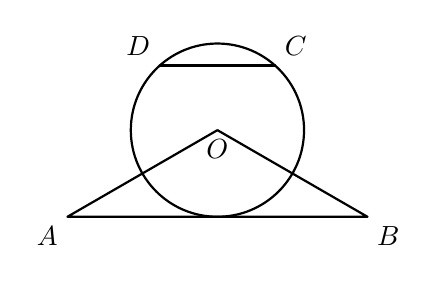
\begin{tikzpicture}[line cap=round,line join=round]
\coordinate (O) at (0,0);
\coordinate (A) at (-1.905,-1.1);
\coordinate (B) at (1.905,-1.1);
\coordinate (D) at (-0.733,0.82);
\coordinate (C) at (0.733,0.82);

\draw[thick] (O) circle (1.1);
\draw[thick] (O)--(A) (O)--(B) (A)--(B);
\draw[thick] (D)--(C);

\node[below left] at (A) {$A$};
\node[below right] at (B) {$B$};
\node[below] at (O) {$O$};
\node[above left] at (D) {$D$};
\node[above right] at (C) {$C$};
\end{tikzpicture}
\end{center}
\nopagebreak[4]
   （1）　证明：直线 \(AB\) 与 \(\odot O\) 相切；

   （2）　点 \(C,D\) 在 \(\odot O\) 上，且 \(A,B,C,D\) 四点共圆，证明：\(AB\parallel CD\)。

\Needspace{4\baselineskip}
\textbf{解析}

\gksubpart{(1)}

设 \(OA=OB=R\)。等腰三角形顶角为 \(120^\circ\)，高平分顶角，故 \(O\) 到 \(AB\) 的距离为 \(R\cos60^\circ=R/2\)，恰等于所作圆半径，所以 \(AB\) 与圆相切。

\gksubpart{(2)}

为证平行，取坐标 \(O=(0,0)\)、\(A=(-\frac{\sqrt3R}{2},-\frac R2)\)、\(B=(\frac{\sqrt3R}{2},-\frac R2)\)，小圆方程为 \(x^2+y^2=R^2/4\)。过 \(A,B,C,D\) 的圆心在 \(x=0\) 上，其方程可写成 \(x^2+y^2-2ky+q=0\)。与小圆方程相减，公共弦 \(CD\) 所在直线为定值 \(y\)，即水平线；因 \(C,D\) 为两个交点，不会是同心圆重合的情形，故 \(CD\parallel AB\)。

\gkanswer{答案（1）：\(AB\) 与圆相切}

\gkanswer{答案（2）：\(AB\parallel CD\)}

\end{answer}
\begin{answer}
\gksolhead{23}{}

\textbf{题目}：

\Needspace{5\baselineskip}
在直角坐标系 \(xOy\) 中，曲线 \(C_1\) 的参数方程为
\nopagebreak[4]
\[
\begin{cases}
x=a\cos t,\\
y=1+a\sin t,
\end{cases}\qquad(t\text{ 为参数},\ a>0).
\]
在以坐标原点为极点，\(x\) 轴正半轴为极轴的极坐标系中，曲线 \(C_2:\rho=4\cos\theta\)。

   （1）　说明 \(C_1\) 是哪种曲线，并将 \(C_1\) 的方程化为极坐标方程；

   （2）　直线 \(C_3\) 的极坐标方程为 \(\theta=\alpha_0\)，其中 \(\alpha_0\) 满足 \(\tan\alpha_0=2\)。若曲线 \(C_1\) 与 \(C_2\) 的公共点都在 \(C_3\) 上，求 \(a\)。

\Needspace{4\baselineskip}
\textbf{解析}

\gksubpart{(1)}

\Needspace{5\baselineskip}
消去参数得 \(x^2+(y-1)^2=a^2\)，所以 \(C_1\) 是圆心 \((0,1)\)、半径 \(a\) 的圆。代入 \(x=\rho\cos\theta,\ y=\rho\sin\theta\)，得极坐标方程
\nopagebreak[4]
\[
\rho^2-2\rho\sin\theta+1-a^2=0.
\]

\gksubpart{(2)}

\Needspace{5\baselineskip}
\(C_2:\rho=4\cos\theta\) 化为直角坐标方程 \((x-2)^2+y^2=4\)，圆心为 \((2,0)\)、半径为 \(2\)。两圆圆心距为 \(\sqrt5\)，相减所得根轴为
\nopagebreak[4]
\[
y=2x+\frac{1-a^2}{2}.
\]
直线 \(C_3\) 为 \(y=2x\)。若另加“\(C_1,C_2\) 有非空公共点”的前提，则两个交点都在 \(C_3\) 时根轴与 \(C_3\) 重合，得到 \(a=1\)；相切时公共点也须为 \(C_2\cap C_3\) 上的点，这两点到 \((0,1)\) 的距离均为 \(1\)，仍得 \(a=1\)。

原卷只写“公共点都在 \(C_3\) 上”，未明示交集非空。若 \(C_1,C_2\) 不相交，该全称条件按字面空真；不相交还允许 \(0<a<\sqrt5-2\) 或 \(a>\sqrt5+2\)。因此按原文不能确定唯一的 \(a\)，本小问标 U，见 ISSUE-0932。

\gkanswer{答案（1）：圆心 \((0,1)\)、半径 \(a\) 的圆；\(\rho^2-2\rho\sin\theta+1-a^2=0\)}

\gkanswer{答案（2）：U；若另加 \(C_1\cap C_2\ne\varnothing\)，则 \(a=1\)。见 ISSUE-0932}

\end{answer}
\begin{answer}
\gksolhead{24}{}

\textbf{题目}：

已知函数 \(f(x)=|x+1|-|2x-3|\)。

   （1）　在图中画出 \(y=f(x)\) 的图象；

   （2）　求不等式 \(|f(x)|>1\) 的解集。
\nopagebreak[4]
\begin{center}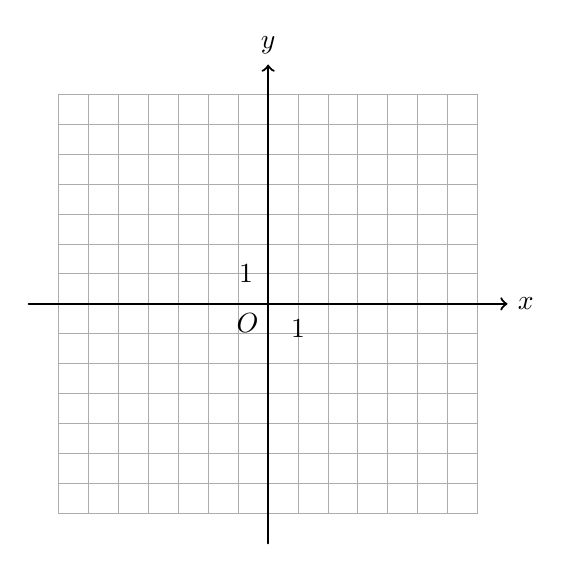
\begin{tikzpicture}[x=0.38cm,y=0.38cm,line cap=round,line join=round]
\foreach \x in {-7,-6,...,7} {
  \draw[gray!65,line width=0.35pt] (\x,-7) -- (\x,7);
}
\foreach \y in {-7,-6,...,7} {
  \draw[gray!65,line width=0.35pt] (-7,\y) -- (7,\y);
}
\draw[->,thick] (-8,0) -- (8,0) node[right] {$x$};
\draw[->,thick] (0,-8) -- (0,8) node[above] {$y$};
\node[below left] at (0,0) {$O$};
\node[left=2pt] at (0,1) {$1$};
\node[below=2pt] at (1,0) {$1$};
\end{tikzpicture}
\end{center}
\nopagebreak[4]
\Needspace{4\baselineskip}
\textbf{解析}

\gksubpart{(1)}

\Needspace{5\baselineskip}
按绝对值分段，
\nopagebreak[4]
\[
f(x)=\begin{cases}
x-4,&x<-1,\\
3x-2,&-1\le x<\frac32,\\
4-x,&x\ge\frac32.
\end{cases}
\]
图象由三段直线组成，连接点为 \((-1,-5)\) 与 \((\frac32,\frac52)\)，据此在题图网格中作图。

\gksubpart{(2)}

由 \(|f(x)|>1\) 分段求解：第一段全满足；第二段解得 \([-1,\frac13)\cup(1,\frac32)\)；第三段解得 \([\frac32,3)\cup(5,+\infty)\)。合并并注意边界处函数值，解集为 \((-\infty,\frac13)\cup(1,3)\cup(5,+\infty)\)。

\gkanswer{答案（1）：$f(x)=\begin{cases}x-4,&x<-1,\\3x-2,&-1\le x<\frac32,\\4-x,&x\ge\frac32\end{cases}$}

\gkanswer{答案（2）：\((-\infty,\frac13)\cup(1,3)\cup(5,+\infty)\)}

\end{answer}